\documentclass{nitk} 
\usepackage{fullpage}

\usepackage{amsmath}
\usepackage[parfill]{parskip}
\usepackage{blindtext, graphicx}
\usepackage{float}
\usepackage{pgfgantt}
\usepackage{algorithm}
\usepackage[noend]{algpseudocode}

\makeatletter
\def\BState{\State\hskip-\ALG@thistlm}
\makeatother

\usepackage[T1]{fontenc}
\usepackage{tikz}
\usetikzlibrary{arrows,calc,positioning}


\usepackage{graphicx}
\usepackage{subfig}
\usepackage{booktabs}

% The document class to be used is nitk.
% Internally, it is an extension of the LaTeX article class.

\report{Project Report} % What report is this?
\title{Query Expansion and Pseudo-Relevance feedback using Firefly Algorithm} % What is the title of the report?
% \rollno{14IT103}
\author{
    \textrm{15IT141 Shamitha S Udupa \and \vspace{-0.25cm}
   	15IT239 Sanjana B}
}

\guide{Dr Sowmya Kamath S} % Who is the guide? Or who are you submitting this work to?
\dept{Dept. of Information Technology} % What is the department you are submitting the report to?
\years{2017-2018}
\place{Surathkal,Nitk} % The place to be used in the declaration.
	\begin{document}
    \maketitle
    \newpage
    \pagenumbering{gobble}
    \begin{center}
    \textsc{\Large{Department of Information Technology}}
    \textsc{\Large{Nitk Surathkal}}
    
    \vspace{5mm}
    \textbf{\large{End Semester Evaluation(May 2018)}}
    \noindent\rule{16cm}{0.2pt}
    \end{center}

	
    \noindent
    \textbf{Course Code : } IT362
    \textbf{Course Title : } Information Retrieval
    \textbf{Project Title : } Query Expansion and Pseudo-Relevance feedback using Firefly Algorithm
    \subsection*{Project Group:}
    \begin{tabular}{lcl}
    \hline
    Name of the student &Register Number &Signature with date \\
    \hline
    \\
    Shamitha S Udupa &15IT141 &  \\\\
    Sanjana B &15IT239	& 
    \\\\
    \hline
    \end{tabular}
    \vspace{5 em}

    Place:

    Date:\hfill \textit{(Name and Signature of Mini Project Guide)}
	
    \newpage
    \abstract{The hardship in finding keywords used in the search queries which are incomplete or not precise has resulted in search engines failing to retrieve the relevant information. A promising  technique to escape this hurdle and improvise the search engine's performance is Query Expansion, wherein the original query of user is altered by adding new terms that characterize the user's information needs in the best way and produce a better query. To enhance the effectiveness of retrieval of query expansion along with low calculation cost,an evolutionary algorithm based on Firefly behaviour is used. In contrast to the traditional methods, the Firefly Algorithm finds the best expanded query from among fireflies representing expanded query solutions instead of selecting the expansion terms which are best. In this approach the length of the expanded query is determined using experimental evaluation. Experiments have been performed on the MEDLINE dataset, the online medical database.The results indicate that the firefly approach is more effecient when compared to existing architectures.}
\makedeclaration{We hereby declare that the project entitled \textbf{\textit{``Query Expansion and Pseudo-Relevance feedback using Firefly Algorithm''}} was carried out by us during the even semester of the academic year 2017 -- 2018. We declare that this is our own work and it has been completed successfully according to the direction of our guide Prof Dr Sowmya Kamath S and as per the specifications of Department of Information Technology, NITK Surathkal.}     
\acknowledge{We would like to express our gratitude to our mini project guide Prof Dr Sowmya Kamath S whose scholarly guidance and suggestions have helped us to carry out the present research work.
We thank the Department of Information Technology for granting us with necesarry department server access to carry out the experimental evaluation of our project.
}
\tableofcontents
\listoffigures
\listoftables
\listofalgorithms
\newpage
\pagenumbering{arabic}
\section{Introduction}
In recent times,the amount of available information online has been growing tremendously. Amount of user generated media is increasing tremendously on social media platforms. The unprecedented growth of information has led to addition of new words, first occurences of names,acronyms,abbreviations,emoticons and so on.\cite{chen} have indicated that most of the query keywords are not in general vocabulary,or are abbreviated speeches(eg: BRB),proper names or wrong spellings or foreign words.

The hardship of finding these new imprecise,ambiguous words results in poor retrieval of information in search engines. Query expansion is a promising technique to overcome this problem.
In QE,query is improvised by adding new key words to it that capture the user's information need better or produce a more useful query. 

Currently, QE is a very promising technique to increase the effectiveness of retrieval. In recent times several new query techniques have been proposed nonetheless the results from these works are not significantly different from state-of-art techniques.

The main reason for the above drawback is that these techniques rely on traditional methods which search for best suited query terms and not best expanded query.We can try to tackle this problem by thinking of selection of the best expanded query as an optimisation problem.

Complete optimisation problems are np-hard and no polynomial time algorithms exist. For practical purposes, these methods might not be optimal. Thus approximate solutions to solve combinatorial optimisation problems have received more attention.Evolutionary algorithms are such algorithms which might give up the guarantee of finding the best solution but always give good solutions with less computation.

Firefly algorithms in 2008 \cite{yang1},\cite{yang2} is based on the phenomenon of bioluminescent communication and the flashing behavior of fireflies. 
 An original approach for finding pseudo-relevance and query expansion based on Firefly algorithm is proposed. We evaluate this approach using Medline Dataset and query expansion techniques, rocchio\cite{Rocchio} and Robertson/Spark Jones\cite{rsj} technique are used as the baseline for comparison.
\newpage
\section{Literature Review}
\subsection{Background}
The increase in size of new queries such as first occurences from proper names, abbreviations, misspelling words and use of ambiguous and imprecise words to describe the information need have caused failure of information retrieval matching the corresponding need.Several methods such as  including search result clustering, concept based lattice IR and contextual document ranking modeled as basis vectors have been proposed to overcome this. Expansion of  the user's query by appending extra relevant keywords is still a promising technique to enhance the effectiveness of the IR system's retrieval.
 
\subsection{Outcome of Literature Review}
One well-known approach is Pseudo-Relevance Feedback(PRF).Pseudo-relevant documents i.e. the initial set of documents retrieved w.r.t original query are used to choose the terms that can be used as expansion keywords.\cite{PRF} As shown in the Figure~\ref{fig:prf} the pseudo-relevance feedback performs a search for the original query. The documents are scored and ranked using Okapi BM25 \cite{okapi}. The top-ranked documents are taken as  pseudo-relevant documents. The vocabulary of the pseudo relevant documents are ranked using Robertson/Sparck Jones or Rocchio's to get best expansion keywords. Finally, the expansion query is got  by adding the top-ranked keywords to original query. Pseudo-Relevance Feedback provides a more precise description of the query but it doesnot look for a suitable expanded query.
\begin{figure}[!htb]

\tikzstyle{intg}=[draw,minimum size=3em,text centered,text width=6.cm]
    \centering
    \begin{tikzpicture}[
      >=latex',
      auto
    ]
    \node[intg] (s) {Start};
    \node [intg] (kp) [node distance=2cm,below of=s]{Read the original query};
    \node [intg] (kp1) [node distance=2cm,below of=kp]{Retrieve and rank the pseudo-relevant documents using Okapi-BM25};
    \node [intg] (kp2) [node distance=2cm,below of=kp1]{Extract and rank the expansion keywords using term-scoring function(RSJ,Rocchio's weight)};
    \node [intg] (kp3) [node distance=2cm,below of=kp2]{Add the top ranked keywords to the original query};
    \node [intg] (kp4) [node distance=2cm,below of=kp3]{Retrieve and rank the relevant documents};
    \node [intg] (kp5) [node distance=2cm,below of=kp4]{End};
    \draw[->] (s) -- (kp);
    \draw[->] (kp) -- (kp1);
    \draw[->] (kp1) -- (kp2);
    \draw[->] (kp2) -- (kp3);
    \draw[->] (kp3) -- (kp4);
    \draw[->] (kp4) -- (kp5);
    
    
  \end{tikzpicture}
  

\caption{Pseudo-Relevance Feedback}
\label{fig:prf}
\end{figure}
Further, \cite{Rocchio} proposes a Rocchio's model based on proximity for pseudo relevance feedback. 
\cite{enhancedprf} attempts to increase PRF by applying a supervised learning method for choosing expansion terms in order to segragate good expansion terms from the rest. They have used  the C-SVM to select the best expansion keywords.

Further,in this method\cite{cluster}, overlapping clusters are formed to find the important documents for the original query's retrieval and repeatedly uses these documents to highlight the important topics of the query.

Particle swarm optimization algorithm can be used to improve PRF by choosing an appropriate combination of term weights in the query vector and a fitness function to measure the proximity between the re-weighted query terms and top ranked documents retrieved by original query. This method although popular,the results are similar to those of the existing techniques.
\subsection{Problem Statement}
"To increase the retrieval effectiveness of pseudo-relevance feedback using firefly algorithm to find the best expanded query while maintaining low cost."

In this project, query expansion is looked from the prespective of expanded query rather than expansion keywords. Swarm optimisation based firefly algorithm is chosen to select the best expanded query from firefly query candidates. An Information Retrieval system is built on the expanded query and documents are ranked by Okapi BM25 model.
\subsection{Objectives}
1. To construct the inverted index for MEDLINE dataset

2. An Information Retrieval system for effective retrieval of documents using Okapi BM25 model

3. Implementation of Firefly algorithm to find the expanded query

4. Evaluation of the retrieval effectiveness using different measures like Precision and Mean Average Precision(MAP)

5. Comparison of our system with the PRF based on Rochhio's weight and Robertson/Sparck Jones weight to find best expansion keyword 
\newpage
\section{Methodology}
We will now discuss Firefly algorithm based approach. As shown in Figure~\ref{fig:flowchart} the procedure consists of getting the pseudo-relevant documents and respective terms to build p solution and executing the algorithm to derive the expanded query.
\begin{figure}[!htb]

\tikzstyle{intg}=[draw,minimum size=3em,text centered,text width=6.cm]
    \centering
    \begin{tikzpicture}[
      >=latex',
      auto
    ]
    \node[intg] (s) {Start};
    \node [intg] (kp) [node distance=2cm,below of=s]{Read the original query};
    \node [intg] (kp1) [node distance=2cm,below of=kp]{Retrieve and rank the pseudo-relevant documents using Okapi-BM25};
    \node [intg] (kp2) [node distance=2cm,below of=kp1]{Select the best expanded query using Firefly algorithm};
    \node [intg] (kp3) [node distance=2cm,below of=kp2]{Retrieve and rank the relevant docs};
    \node [intg] (kp4) [node distance=2cm,below of=kp3]{End};
    \draw[->] (s) -- (kp);
    \draw[->] (kp) -- (kp1);
    \draw[->] (kp1) -- (kp2);
    \draw[->] (kp2) -- (kp3);
    \draw[->] (kp3) -- (kp4);
    
    
  \end{tikzpicture}
  

\caption{The proposed Firefly Algorithm for prf}
\label{fig:flowchart}
\end{figure}
\subsection{Solutions' representation and initialisation of population}
Each solution is represented by a firefly with the search space consisting of all of fireflies generated.Although a firefly in our problem would be the expanded query, we only consider the additional terms for optimisation concern.
\begin{equation}
\label{eq:vector}
\begin{aligned}
\tilde{Q} = < \tilde{q_1},\tilde{q_2},....,\tilde{q_{|\tilde{Q}|}} >
\end{aligned}
\end{equation}
\begin{equation}
\label{eq:expq}
\begin{aligned}
	EQ = Q + \tilde{Q}
\end{aligned}
\end{equation}
Equation~\ref{eq:vector} is a vector representation of the terms that can be appended to the original query. The overall expanded query is given by Equation ~\ref{eq:expq}.

The search space has all potential fireflies vocabulary.The size of the search space consists of all possible combinations from vocabulary of pseudo relevant documents with $|$\~{Q}$|$(length of vector \~{Q}). Thus the solution space order is of the binomial of the coefficient of the above mentioned vocabulary and $|$\~{Q}$|$. This huge number describes the numerous possibilities that can be exploited to build a query expansion. Regarding the initialisation of population N fireflies are chosen randomly by selecting $|$\~{Q}$|$ terms from the vocabulary of pseudo relevant documents chosen.
The size of pseudo-relevant documents considered has to be determined emperically. 
\subsection{Fitness Function}
The objective function evaluates the solution's quality. Solution means an expanded query,therefore its performance can be assessed by considering the inverted indexes of its terms and then calculating the each document's score such that it belongs to R(pseudo relevant document corpus).
Equation ~\ref{eq:fitness} calculated by pseudo-code in Algorithm ~\ref{algo:fitness} gives the fitness function score for every firefly. 

\begin{equation}
\label{eq:fitness}
\begin{aligned}
f(EQ) = max(score_{bm25}(d1,EQ),score_{bm25}(d2,EQ),...score_{bm25}(d_{\|R\|}))
\end{aligned}
\end{equation}
\begin{algorithm}
\caption{Fitness function pseudocode}
\label{algo:fitness}
\begin{algorithmic}[1]
\Procedure{Fitness function f(EQ)}{}
\State $\text{Inverted index} In(\tilde{q_i})$
\State $\text{Initialise the vector of scores }\textit{S} \gets \text{[ ]}$
\For {\text{each keyword } \textit{\~{qi} } \text{in} \textit{ \~{Q} :}}
\For {\text{each document} \textit{d} \text{in} \textit{R}}
	\If {\text{d E } In(\~{qi}) \text{and S[ d ] != 0} }
    \State $\textit{S[d]} \gets \textit{scorebm25(Q) + scorebm25(\~{Q})}$
    \EndIf end if
\EndFor end for
\EndFor end for
\State $\text{f(EQ)} \gets \text{max(S)}$
\EndProcedure
\end{algorithmic}
\end{algorithm}
Algorithm ~\ref{algo:fitness} initially generates the inverted index of every expansion term \~{qi} belongs to \~{Q} then iteratively calculates each document's score  included in both In and R with respect to the expanded query EQ. The okapi score of \~{Q} is calculated only as the score of Q will already have been calculated.Once the scores have been evaluated,max(S) is the expanded query EQ's fitness value.
As the QE issue is formulated as maximisation problem in Algorithm ~\ref{algo:fitness},the fitness function expresses the light intensity. 
\subsection{Update locations of fireflies}
\begin{equation}
\label{eq:beta}
\begin{aligned}
\beta = 1 \div (1 + \gamma * r_{ij})
\end{aligned}
\end{equation}
The solution differs across the iterations with its fitness function score increasing.The global is compared with the best solution of each iteration and is assigned the local best solution if it has a higher fitness value.
There are two parts to movement of the fireflies.
The first part is determined by Equation~\ref{eq:beta} where :
\newline
$\beta$ belongs to [0,1], indicates the attractiveness of firefly j;
\newline
$\gamma$ indicates the light absorption coefficient;
\newline
$r_{ij}$ indicates the distance or how far firefly i,j are
\newline
The distance is calculated using Hamming distance shown in Equation~\ref{eq:hamming}.The Hamming
distance is the number of elements which do not correspond with each other in the sequence between two fireflies.
\begin{equation}
\label{eq:hamming}
\begin{aligned}
\tilde{W_1} = < \tilde{w_5},\tilde{w_4},\tilde{w_3} >
\tilde{W_2} = <\tilde{w_5},\tilde{w_2},\tilde{w_1}>
\text{Then hamming distance is 2} 
\end{aligned}
\end{equation}
\begin{equation}
\label{eq:beta q}
\begin{aligned}
    \tilde{Q}^{t+1}= 
    \begin{cases}
    \tilde{Q}_{ik}^t, &\text{rand > } \beta \\
    \tilde{Q}_{jl}^t, &\text{otherwise}    
    \end{cases}    
\end{aligned}
\end{equation}
Equation~\ref{eq:beta q} gets the firefly \~{Qi} nearer to a more suitable and attractive solution \~{Qj}. Next the distance between the two fireflies decreases and the attractiveness value is increased.Here
\newline
\newline
$\tilde{Q}_{ik}^t$ doesnot belong to $\tilde{Q}_{j}$, is a term of $\tilde{Q}_i$
\newline
$\tilde{Q}_{jl}^t$ doesnot belong to $\tilde{Q}_i$ is a random term of $\tilde{Q}_{j}$
\newline
\newline
Next Equation~\ref{eq:alpha q} is calculated.The randomization parameter $\alpha$ prevents the trapping of solution at local optima.The value is slowly decremented to prevent the algorithm's premature convergance.
\begin{equation}
\label{eq:alpha q}
\begin{aligned}
    \tilde{Q}^{t+1}= 
    \begin{cases}
    \tilde{Q}_{ik}^t, &\text{rand > } \alpha \\
    \tilde{q}_l, &\text{otherwise}    
    \end{cases}    
\end{aligned}
\end{equation}
Based on the $\alpha$'s value,$\tilde{Q}_i$'position is updated by adjusting each of its element $\tilde{Q}_{ik}$ with $\tilde{q}_l$, a randomly selected keyword from the vocabulary of the pseudo relevant documents.
\subsection{Firefly algorithm algorithm pseudocode}
In Algorithm~\ref{algo:firefly},the first step is to set the initial values of the $\gamma$, absorption coefficient and $\alpha$, the randomisation parameter .The starting N populations are then created randomly from the search space.Each firefly $\tilde{Q}$ is initialised by selecting $|\tilde{Q}|$ terms from vocabulary of pseudo relevant documents. The intensity of light of each firefly is calculated by its fitness function value.The local best solution is the best solution of a given iteration.The global best solution will be the solution with the highest fitness value for all iterations prior to given iteration. Every iteration leads to the global best solution being updated if required. As shown in the Equation~\ref{eq:beta q} and \ref{eq:alpha q}, fireflies move towards a more attractive firefly and provide increasingly better solutions.The termination conditions are that the optimised solution doesnot change for a pre-specified duration of iterations or maximum iteration limit is met.Finally when termination conditions are met,the terms from the global best solution are augmented to the Q to get the expanded query EQ. 
 \begin{algorithm}
 \caption{Firefly algorithm pseudocode}
 \label{algo:firefly}
 \begin{algorithmic}[1]
\Procedure{Firefly algorithm}{}
\State {Fitness function f(\~{Q})}
\State $\text{Define light absorption coefficient} \gamma \text{ ,parameter} \alpha $
\State $\text{Light intensity } I_i \text{ at } Q_i \text{ is determined by f(\~Q)} $
\State {Generate an initial population of N fireflies}
\While {\text{t < Maxiter and bestExpandedQuery still changes}}
\For { i in 1 to N}
\For {i in 1 to N}
	\If {\text{f (\~{Qi}) < f (\~{Qj})}}
    \State $\text{Move query firefly \~{Qi} to \~{Qj}}$
    \EndIf end if
   \State{vary attractiveness}
   \State{Evaluate new solutions}
\EndFor end for
\EndFor end for
\State $\text{Rank the fireflies and find the current best firefly}$
\EndWhile end while
\EndProcedure
\end{algorithmic}
 \end{algorithm}
\newpage
\section{Implementation}
 \subsection{Work Done}
 \subsubsection{Dataset}
 In order to test our IR system, we have used MEDLINE dataset. It is the online medical database accessed via the PubMed interface.It contains articles with title, abstract, author names, date of publication, MeSH(Medical Subject Headings).
 \subsubsection{Preprocessing}
 We have extracted the document title, abstract and MeSH terms and preprocessed them with NLP operations like tokenizing,punctuation removal, stemming and stopword removal. The preprocessed document is used to construct an inverted index containing the index terms and postings list.
 \subsubsection{Information Retrieval System}
 We have created an Information Retrieval system using Okapi BM25 model to generate rankings to the query. The similarity score between the query and documents is calculated using the formula - 
\begin{equation}
\label{eq:okapi bm25}
\begin{aligned}
    BM25{(Q,d_j)}= \sum_{t_i \epsilon Q} {log\bigg({\dfrac{N-n_i+0.5}{n_i+0.5}}\bigg)*\bigg({\dfrac{tf}{tf+k\Big((1-b)+b{\dfrac{dl}{avgdl}}\Big)}}\bigg)}
\end{aligned}
\end{equation}
where Q is the query, ${d_j}$ refers to the jth document in the corpus, N( total documents in the collection), ${n_i}$ (the document frequency of the term $t_i$), tf is the term frequency of the term $t_i$, dl and avgdl refers to the document length of $d_j$ and average length of the documents in the corpus respectively, k and b are constants such that 1.2<k<2 and 0.5<b<0.8 .
 \subsubsection{Firefly Algorithm}
 Firefly algorithm is implemented to find the query terms to give best expanded query.
 \begin{figure}[ht]
 \centering
 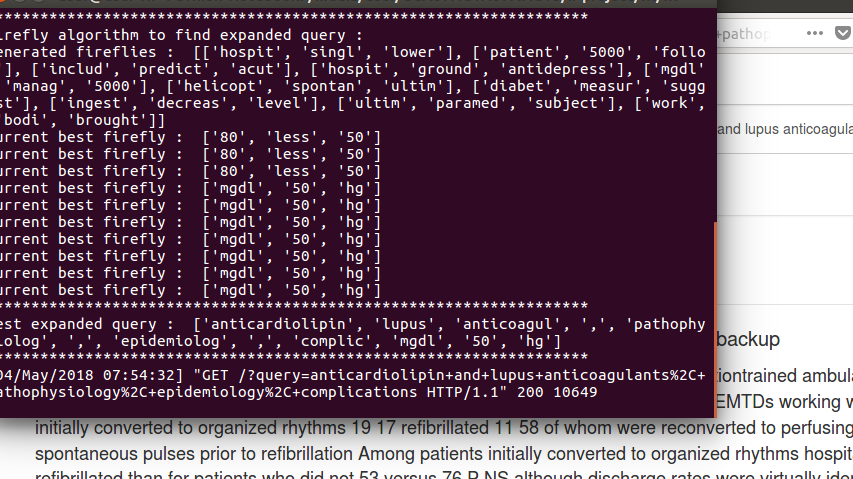
\includegraphics[scale=0.5]{firefly_execution}
 \caption{Firefly algorithm execution}
 \end{figure}
 \subsubsection{Performance Evaluation}
 We have used precision and Mean Average Precision(MAP) evaluation metrics to measure the retrieval effectiveness of our IR system. The results are discussed in the next section.
 \newpage
 \subsection{Result and Analysis}
 \subsubsection{Fixing firefly algorithm parameters}
 In the firefly algorithm we need to emperically find the following parameters - $|\tilde{Q}|$, N and T (the query length, population size and the number of iterations).
 In these primary experiments, these parameters are varied while keeping others constant.The size of |R|(pseudo-relevant documents)  are set as [10,30,50].The parameters $\alpha_0$,$\gamma$ and $\theta$, are tuned at 1,1 and 0.95.
 \begin{figure}[!htb]
 \centering
 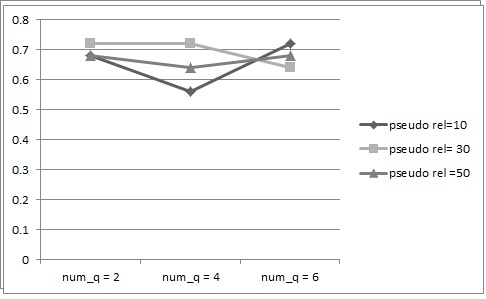
\includegraphics[scale=0.5]{query_length_p_5}
 \caption{P@5 vs varying query length}
 \label{fig:quer_leng_p} 
 \end{figure}
 
 Fig~\ref{fig:quer_leng_p} and Fig~\ref{fig:quer_leng_map} give the P@5 and MAP@10 results after varying $|\tilde{Q}|$ wrt number of query terms [2,4,6]. N and T are kept constant at value 5 and 10 respectively. From the graph we can see that $|\tilde{Q}| = 2 or 4$ gives better results. 
 \begin{figure}[!htb]
 \centering
 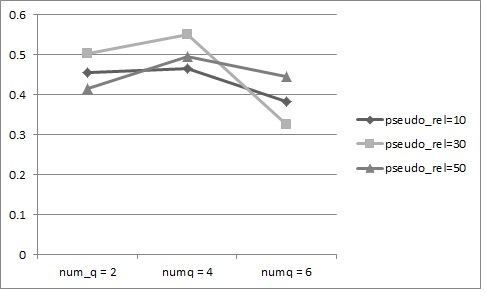
\includegraphics[scale=0.5]{query_length_map_10}
 \caption{MAP@10 vs varying query length}
 \label{fig:quer_leng_map} 
 \end{figure}
 Fig~\ref{fig:pop_p} and Fig~\ref{fig:pop_map} give the P@5 and MAP@10 results for varying population length,N = [5,10,15,20,25]. $|\tilde{Q}|$ and T have values 4 and 10 respectively.
 \begin{figure}[!htb]
 \centering
 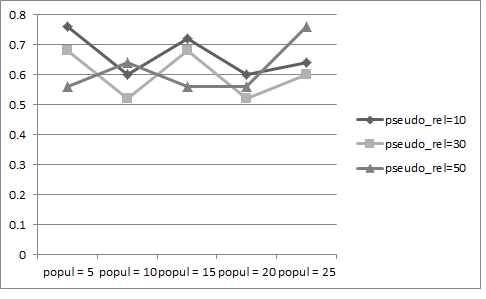
\includegraphics[scale=0.5]{population_p_5}
 \caption{P@5 vs population size}
 \label{fig:pop_p}
 \end{figure}
 \begin{figure}[!htb]
 \centering
 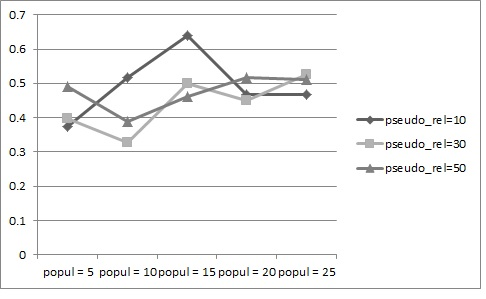
\includegraphics[scale=0.5]{population_map_10}
 \caption{MAP@10 vs varying population size}
 \label{fig:pop_map}
\end{figure}
Fig ~\ref{fig:iter_p} and Fig~\ref{fig:iter_map} give the P@5 and MAP@10 results for varying iterations T =[10,20,30,40,50] while $|\tilde{Q}|$ = 4 and N = 10
\begin{figure}[!htb]
\centering
 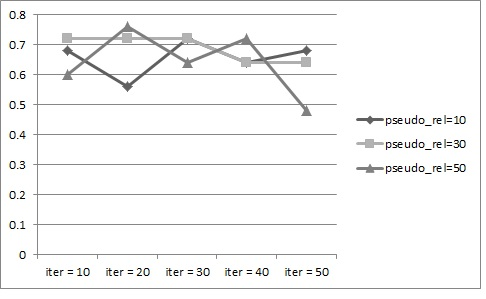
\includegraphics[scale=0.5]{iteration_p_5}
 \caption{P@5 vs number of iterations}
 \label{fig:iter_p}
 \end{figure}
 \begin{figure}[!htb]
 \centering
 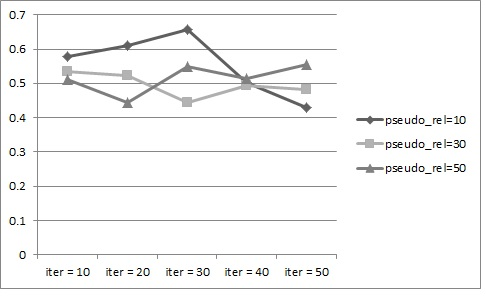
\includegraphics[scale=0.5]{iteration_map_10}
 \caption{MAP@10 vs number of iterations}
 \label{fig:iter_map}
\end{figure}
\subsection{Comparison of Firefly algorithm with Rocchio and RSJ}
\begin{figure}[!htb]
\centering
 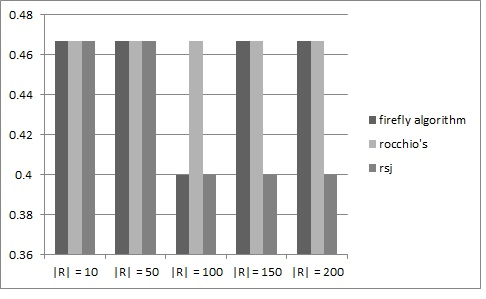
\includegraphics[scale=0.5]{firefly_vs_other}
 \caption{P@5 vs number of iterations}
 \label{fig:frvsoth}
 \end{figure}
Finally we compare the P@5 results of our firefly algorithm with that of Rocchio and RSJ algorithms. N = 10,$|\tilde{Q}|$ = 2, T = 30. The number of pseudo-relevant documents=[10,50,100,150,200]. Fig~\ref{fig:frvsoth} gives the result of above computation.We can see that rocchio and firefly algorithms have almost similar performance and firefly algorithm performs better than rsj algorithm.
\newpage
 \subsection{Innovative Work Done}
 We have developed a web interface which suggests the additional query words that can be added to the improvise the semantic meaning of the query. These additional terms are computed by the firefly algorithm. We have also refined the original query by removing the terms with low values of inverse document frequency(IDF) factor and replacing them with the terms of the global best firefly.
 \begin{figure}[ht]
 \centering
 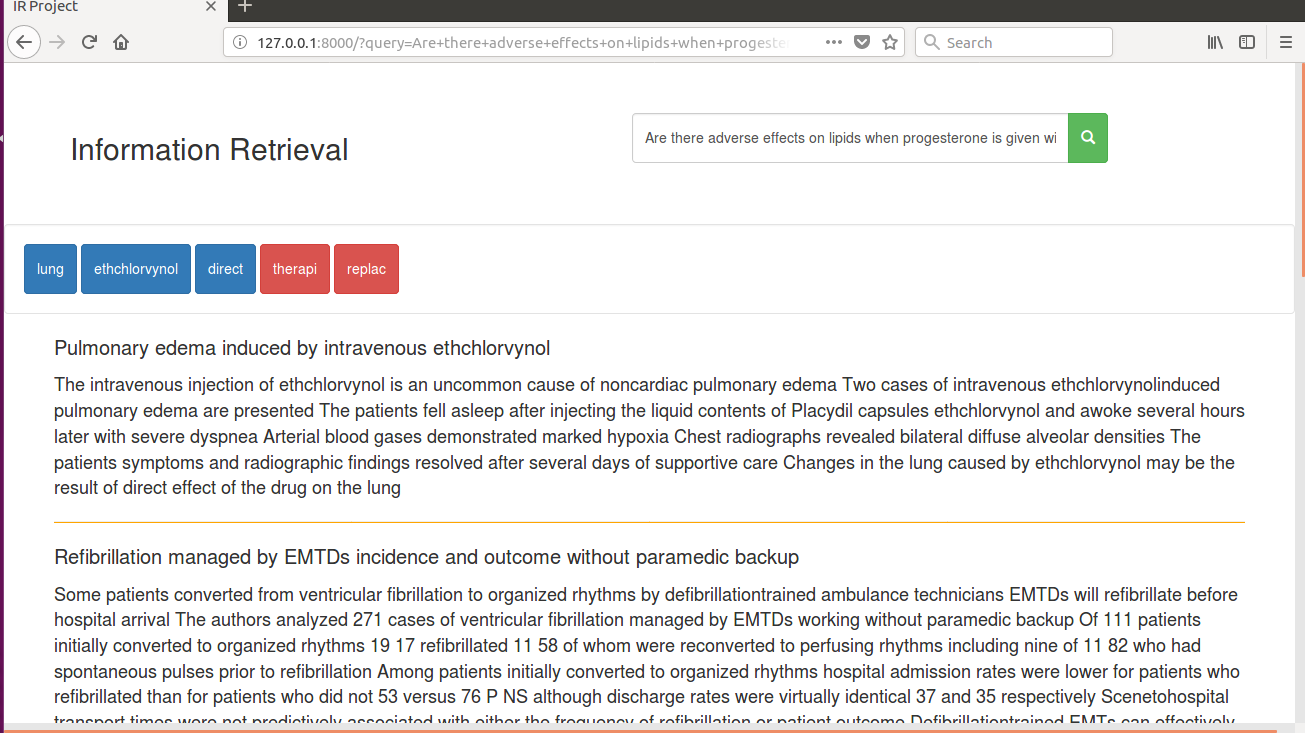
\includegraphics[width=0.8\textwidth,height=0.3\textwidth]{IDF_relevancy}
 \caption{Web Interface for the firefly algorithm}
 \label{fig:web}
 \end{figure}
 In Figure~\ref{fig:web}, the terms in red color are the terms of the original query which have low idf frequency and can be replaced with the terms colored blue calculated by firefly algorithm. 
 \subsection{Individual Work Distribution}
 \begin{figure}[!htb]
\centering
 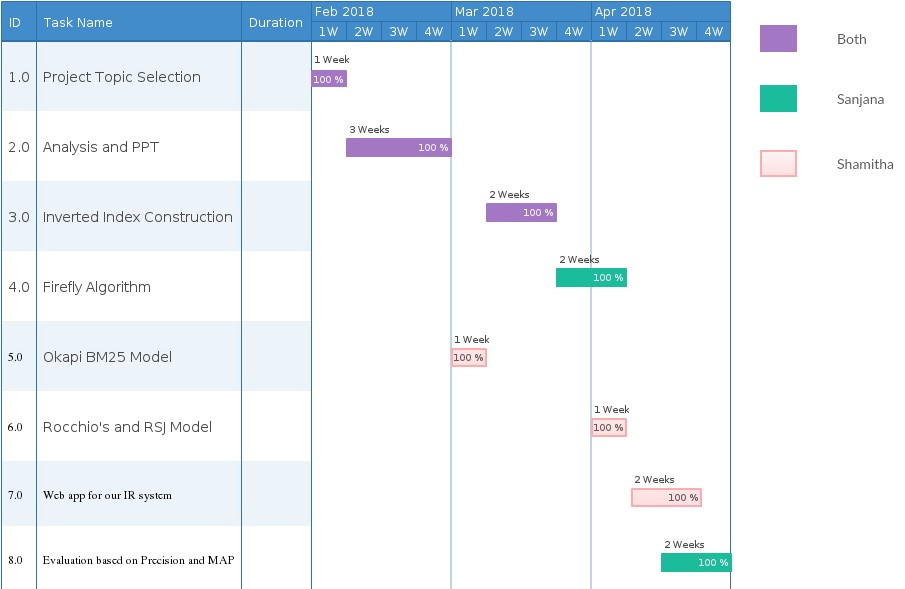
\includegraphics[scale=0.5]{IR_Gantt_Chart_}
 \caption{Gantt Chart}
 \label{fig:GC}
 \end{figure}
 \section{Future Work}
 We will try to improvise the firefly algorithm by designing a parallel variant of the same to increase both efficiency and effectiveness of our IR system. Further we will try to refine the query using automatically generated thesaurus and synsets from WordNet.
\newpage
\bibliographystyle{IEEEtran}
\bibliography{project}
\end{document}
    